\documentclass[11pt,a4paper]{report}
\usepackage[english]{babel}
\usepackage{blindtext}
\usepackage[utf8]{inputenc}

% 1. TeXDoclet output include
\usepackage{color}
\usepackage{ifthen}
\usepackage{ifpdf}
\usepackage[headings]{fullpage}
\usepackage{listings}
\lstset{language=Java,breaklines=true}
\ifpdf \usepackage[pdftex, pdfpagemode={UseOutlines},bookmarks,colorlinks,linkcolor={blue},plainpages=false,pdfpagelabels,citecolor={red},breaklinks=true]{hyperref}
  \usepackage[pdftex]{graphicx}
  \pdfcompresslevel=9
  \DeclareGraphicsRule{*}{mps}{*}{}
\else
  \usepackage[dvips]{graphicx}
\fi

\newcommand{\entityintro}[3]{%
  \hbox to \hsize{%
    \vbox{%
      \hbox to .2in{}%
    }%
    {\bf  #1}%
    \dotfill\pageref{#2}%
  }
  \makebox[\hsize]{%
    \parbox{.4in}{}%
    \parbox[l]{5in}{%
      \vspace{1mm}%
      #3%
      \vspace{1mm}%
    }%
  }%
}
\newcommand{\refdefined}[1]{
\expandafter\ifx\csname r@#1\endcsname\relax
\relax\else
{$($in \ref{#1}, page \pageref{#1}$)$}\fi}
\date{null}
\chardef\textbackslash=`\\


% use behind of TeXDoclet_preamble.tex because of option clash with pdftex
\usepackage{fullpage} 
\usepackage{hyperref}
\hypersetup{
	colorlinks=true,allcolors=blue,pdfpagemode=UseOutlines,pdfpagelayout=TwoPageRight
}
\usepackage{hypcap}

\begin{document}
	
	\date{\today}
	\title{JSynth dokumentáció\bigskip\\ \Large Created with Javadoc TeXDoclet Doclet}
	\author{Szabó Bálint}
	\maketitle
	
	\tableofcontents
	
	\chapter{Specifikáció}
	
	\section{A Feladat}
	A feladat egy olyan program elkészítése, amely különböző hanghullámokat képes generálni, valós időben lejátszani és elmenteni. A felhasználó beállíthatja a hanghullám néhány jellemzőjét, mint például a hangerejét, a generáló függvényt, a lecsengés függvényét, illetve a lecsengés időtartamát.
	\section{Use-case}
	A fontosabb use-case-eket a következő táblázat foglalja össze: \\
	\begin{center}
	\begin{tabular}{|l|p{8cm}|l|}
		\hline
		Név & Leírás & Actor \\ \hline
		Hang leütés & A felhasználó leüt egy billentyűt & Felhasználó \\ \hline
		Generátor váltása & A felhasználó lecseréli a generátor függvényt & Felhasználó \\ \hline
		Lecsengés váltása & A felhasználó lecseréli a lecsengésért felelős függvényt & Felhasználó \\ \hline
		Lecsengés időzítése & A felhasználó beír egy lecsengési időt & Felhasnáló \\ \hline
		Felvétel indítása, leállítása & A felhasználó egy gombbal elindítja vagy leállítja a felvételt, majd elmenti egy fájlba & Felhasználó \\ \hline
		Állapot mentés & A felhasználó elmenti a program beállításait egy fájlba & Felhasználó \\ \hline
	\end{tabular}
	\end{center}
	
	\section{A megvalósítás alapötlete}
	A kezelőfelület SWING-el működik. A hangerőt egy JSlider-en, a generátor és lecsengés függvényeket JComboBox-on, a lecsengés időtartamát JTextField-en lehet beállítani. A felvétel gombbal indítható, az állapot mentése a menüsávból lehetséges.
	A hangok lejátszásáért és felvételéért a Java beépített audio könyvtára felel.
	
	\chapter{A konkrét terv}
	
	\section{Osztálydiagram}
	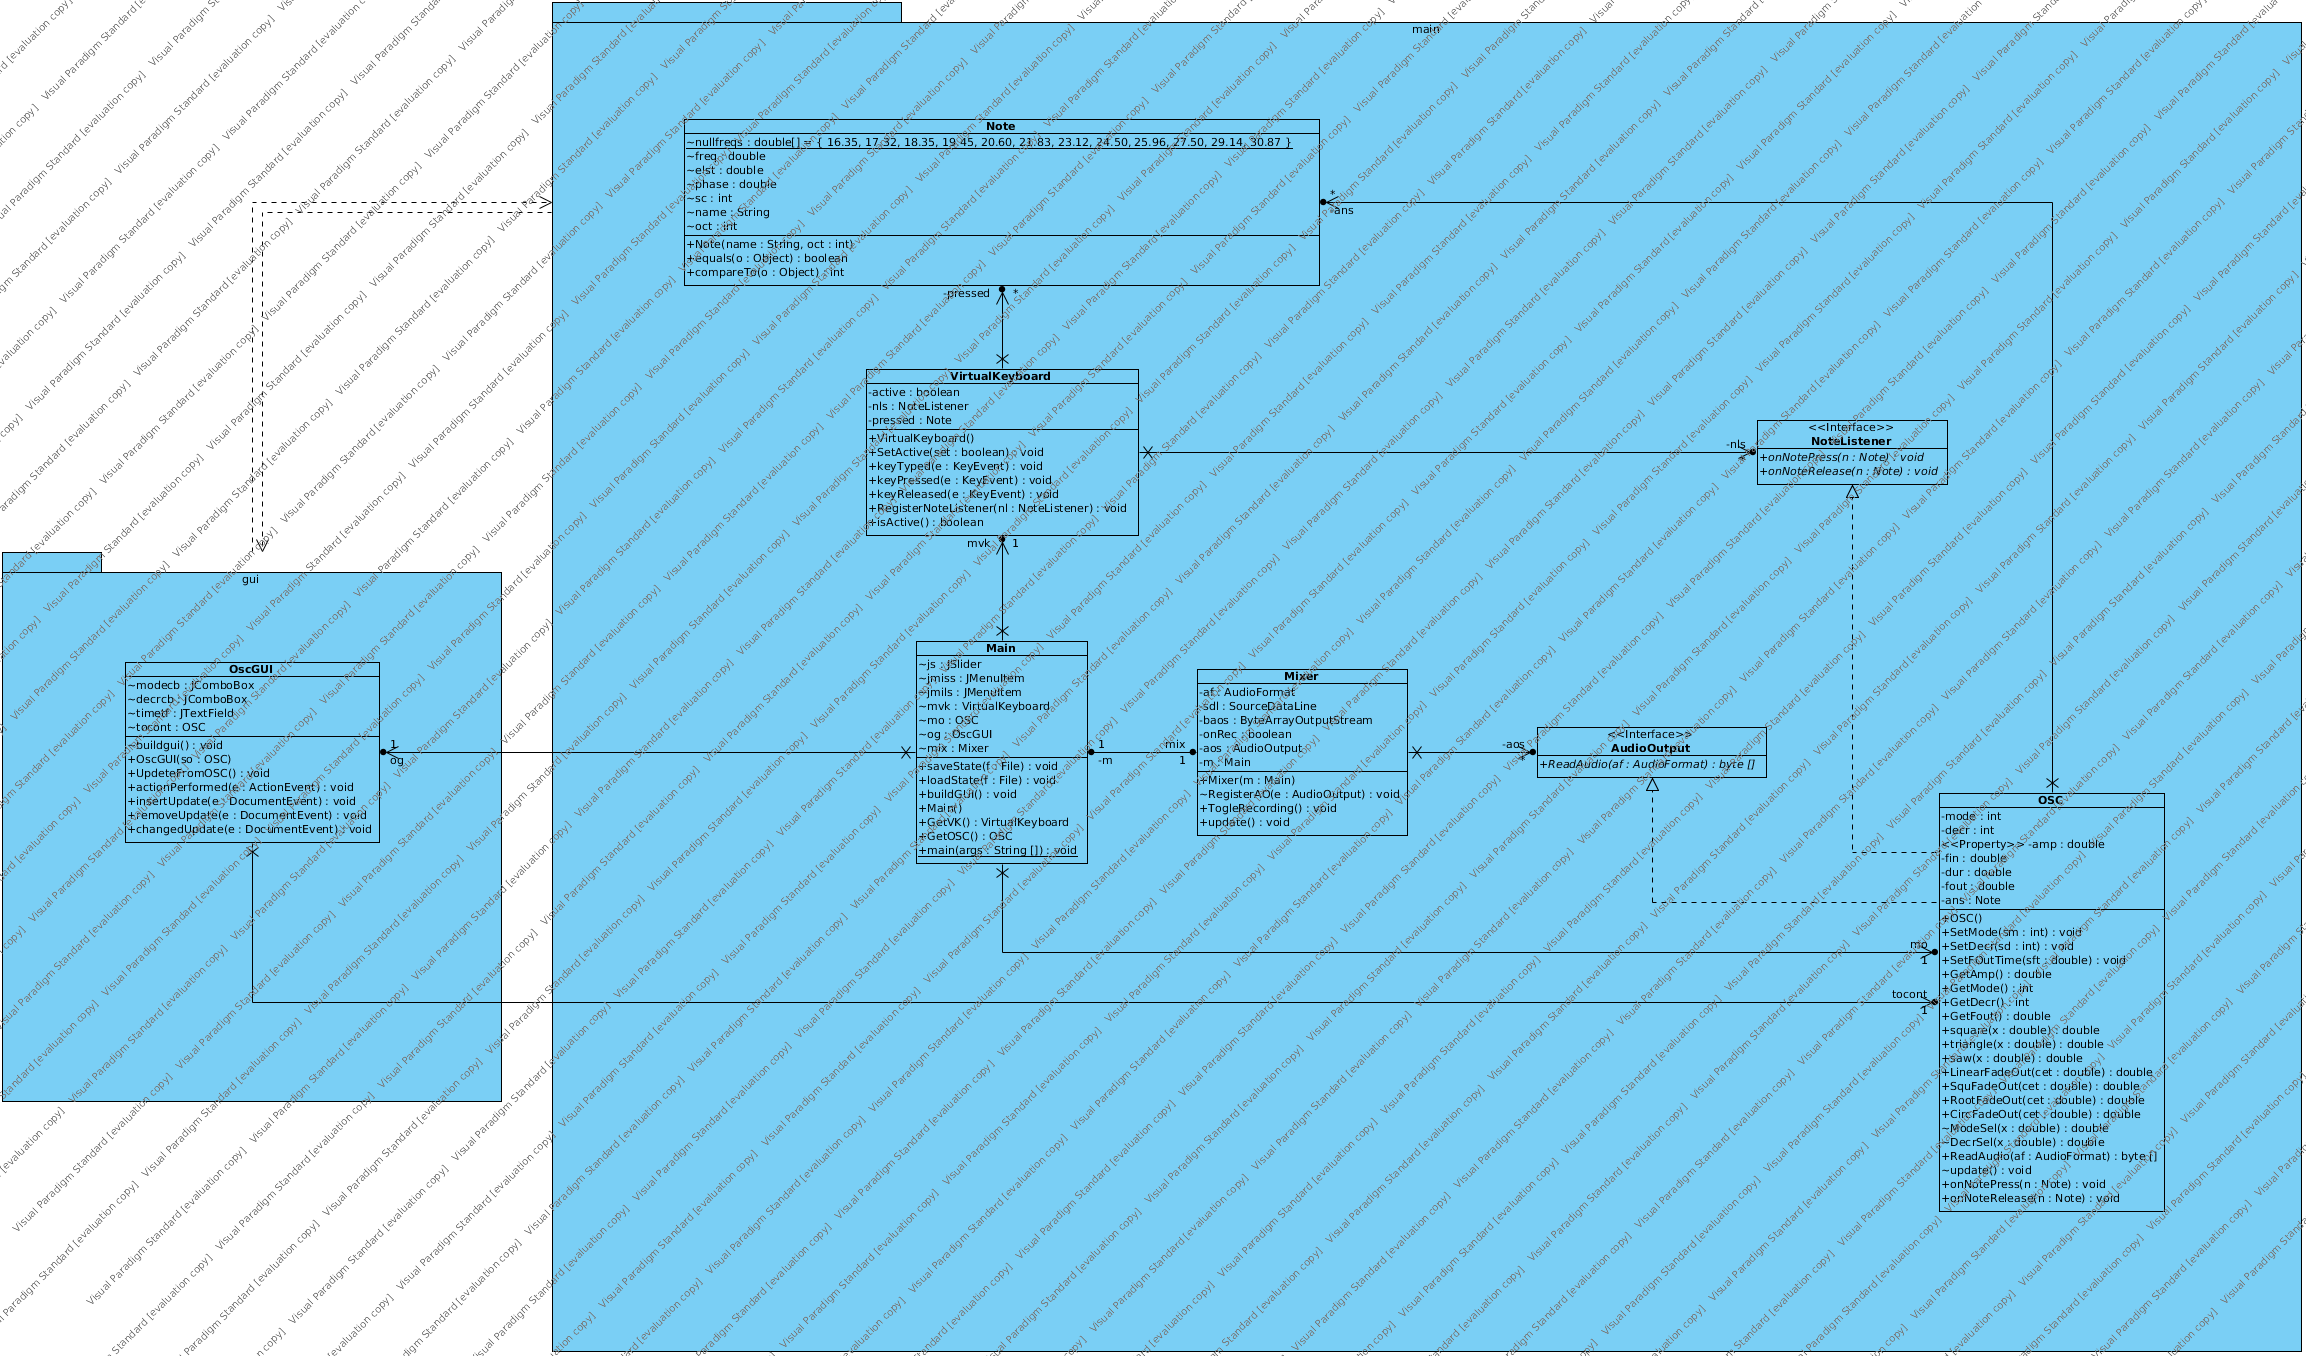
\includegraphics[scale = 0.25]{cdia.png} \\
	
	\section{A lényegesebb funkciók szekvenciái}
	\subsection{A billentyűzet kezelés szekvenciája}
	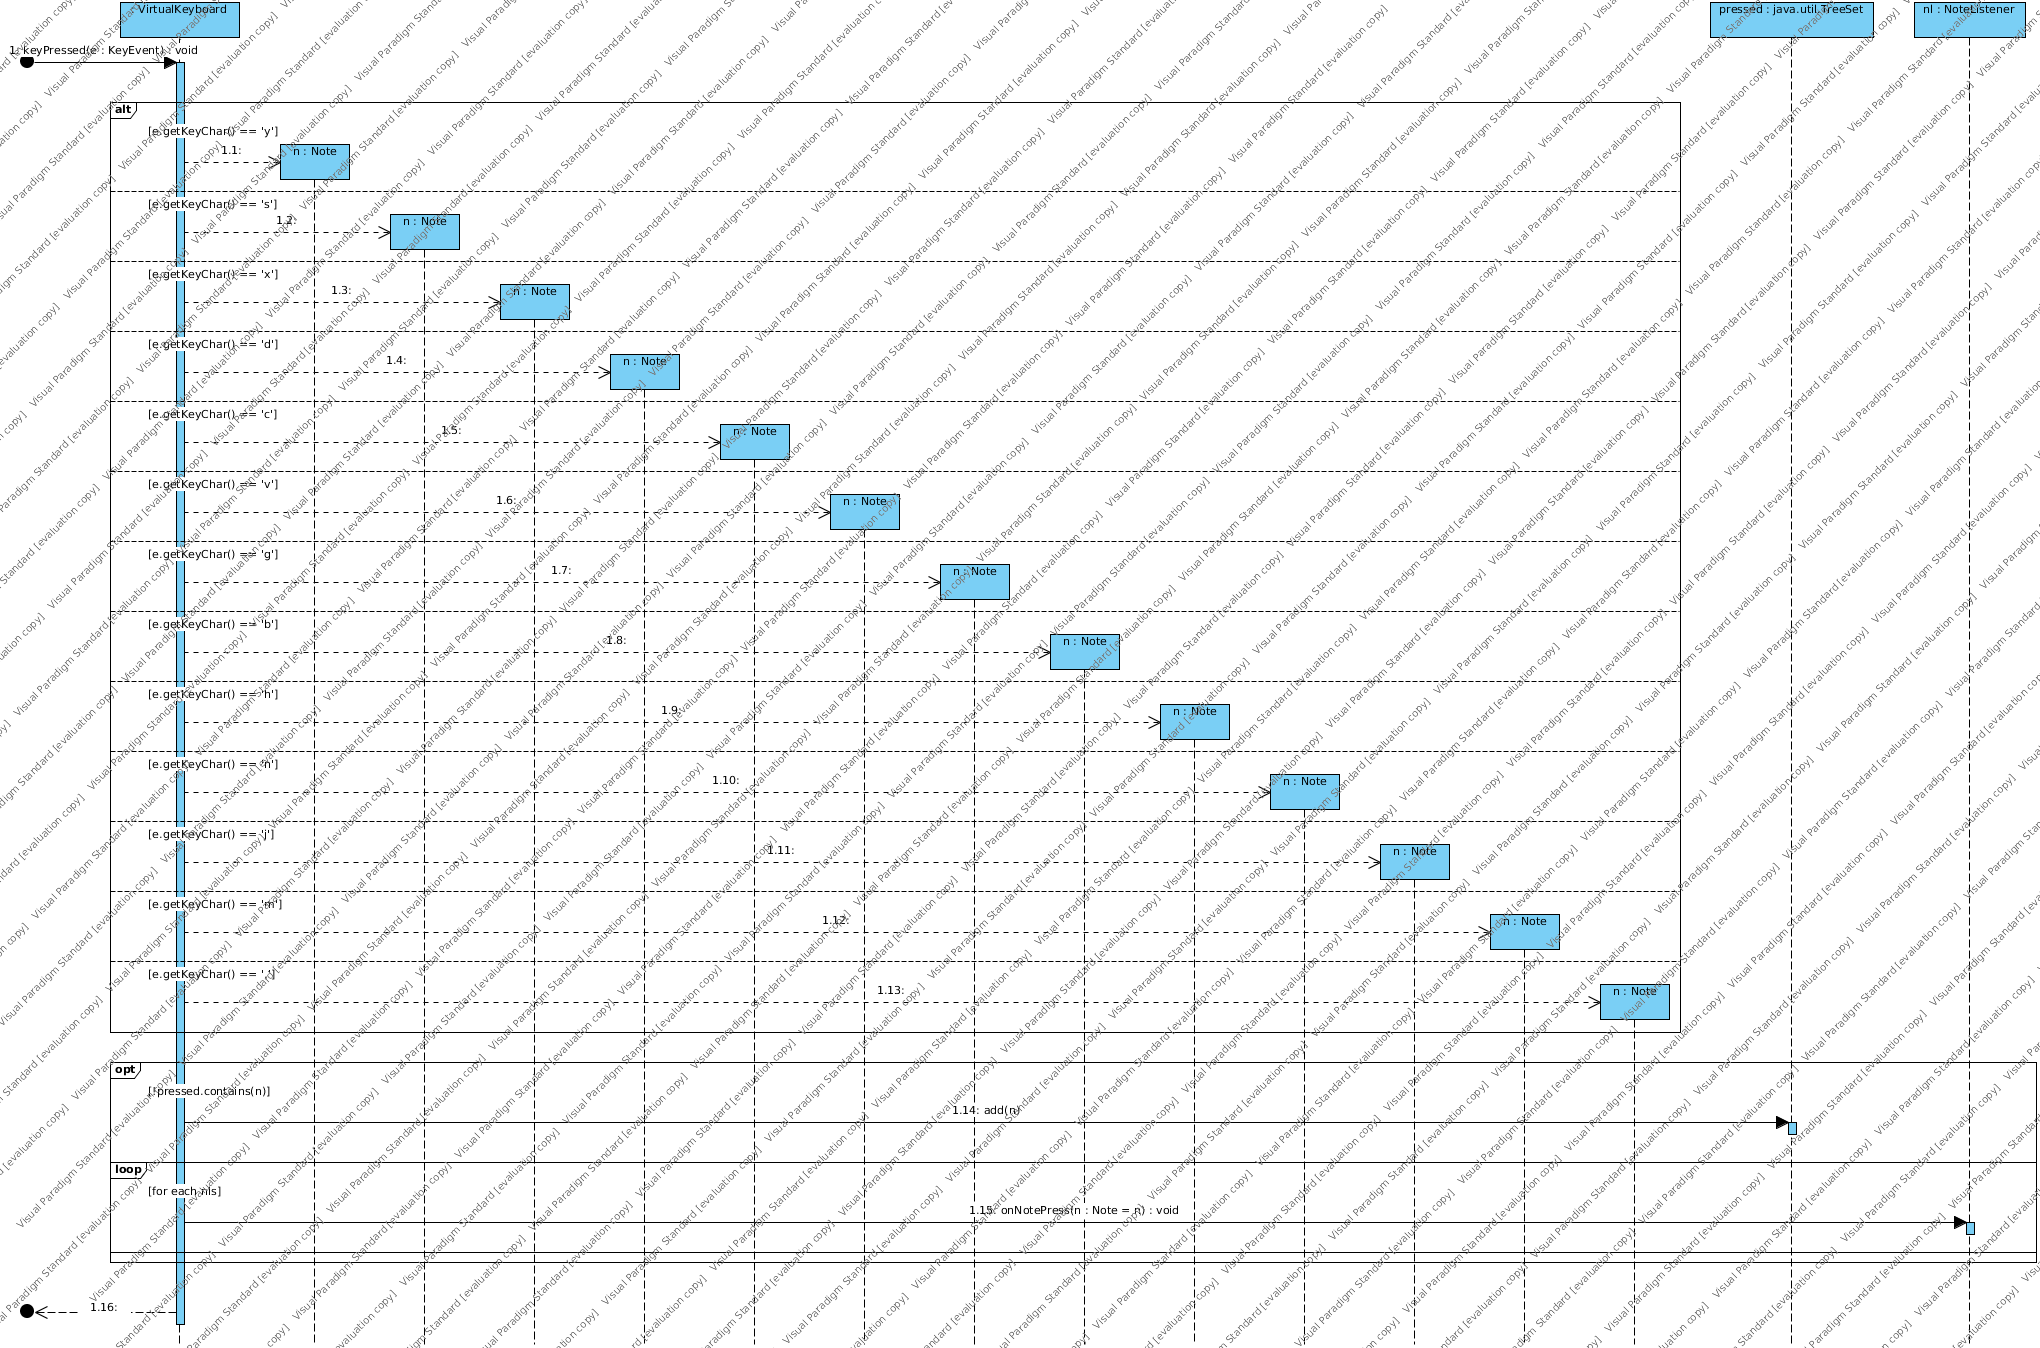
\includegraphics[scale = 0.3]{note.png} \\
	\subsection{A generátor és lecsengető függvények állításának szekvenciája}
	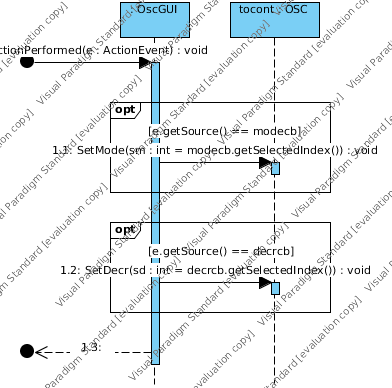
\includegraphics[scale = 0.9]{genlecs.png} \\
	\subsection{A lecsengési idő állítása}
	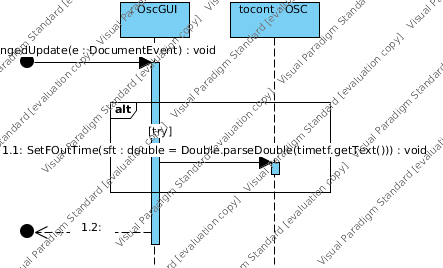
\includegraphics[scale = 0.9]{ido.png} \\
	\subsection{A felvétel indítása, leállítása}
	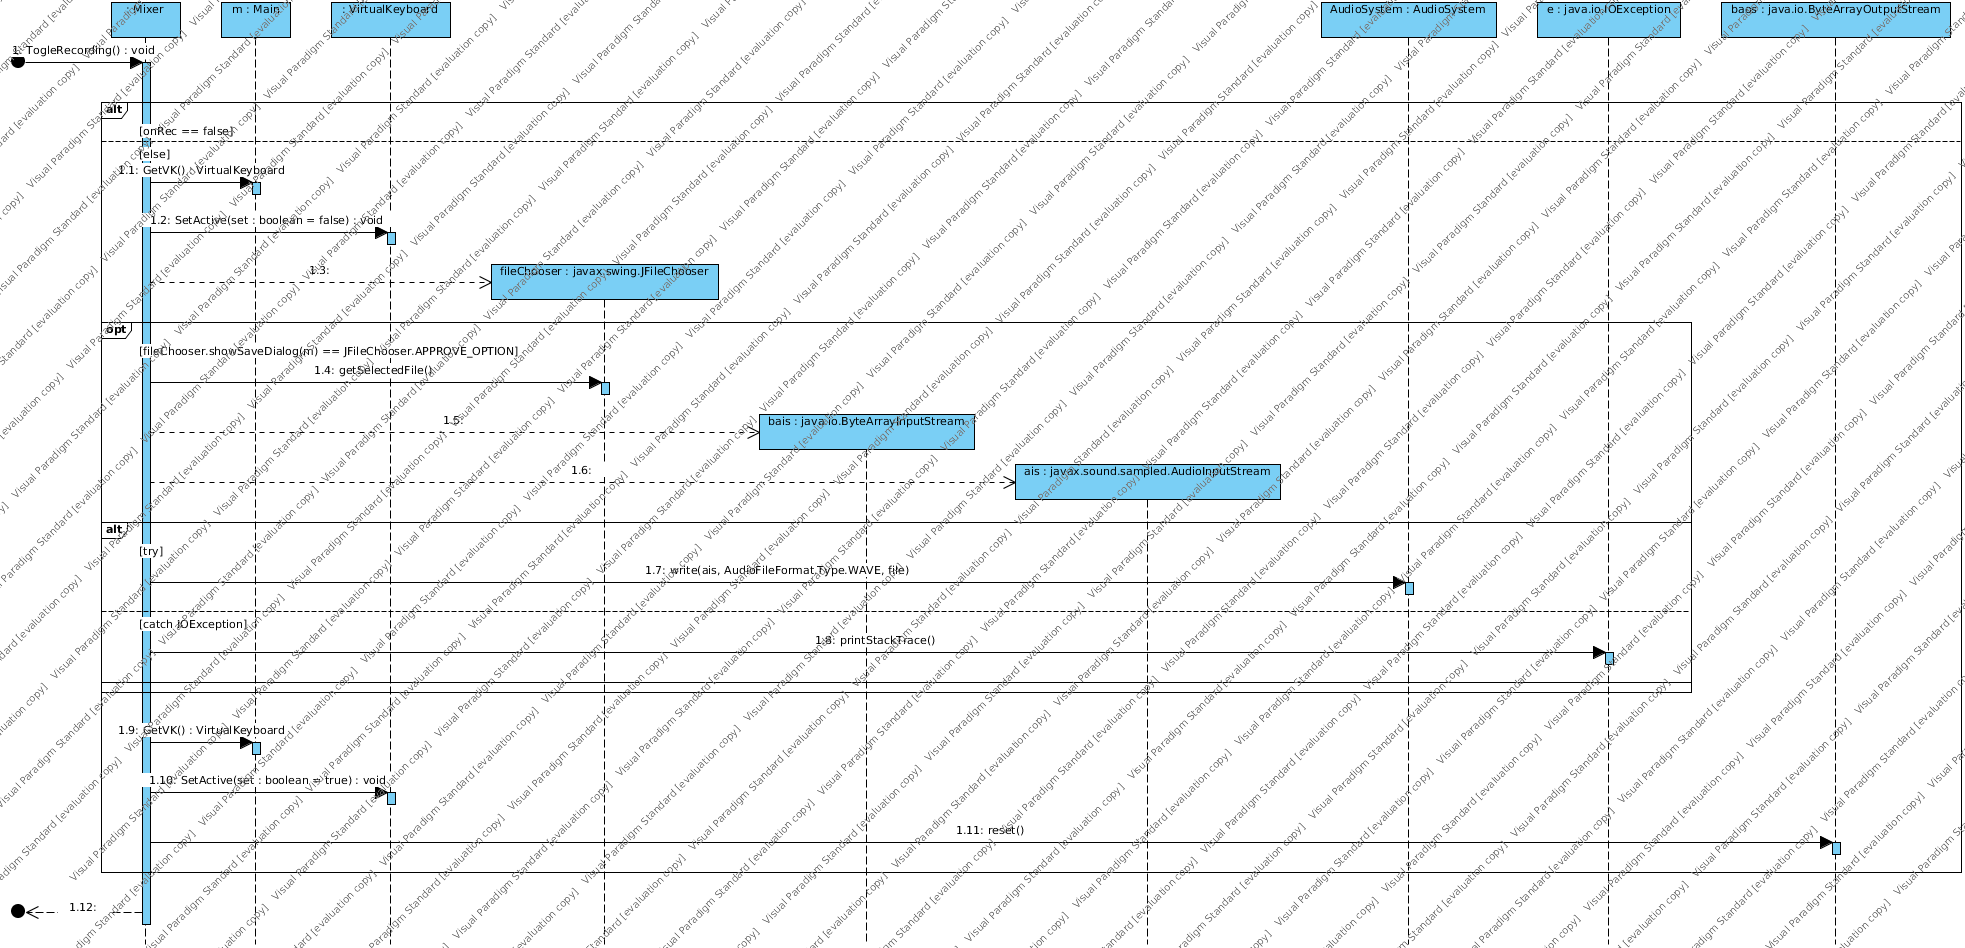
\includegraphics[scale = 0.3]{record.png} \\
	
	
	\chapter{TeXdoclet Java Documentation} {
		% 2. TeXDoclet output include
		\section{Package main}{
\label{main}\hypertarget{main}{}
\hskip -.05in
\hbox to \hsize{\textit{ Package Contents\hfil Page}}
\vskip .13in
\hbox{{\bf  Interfaces}}
\entityintro{AudioOutput}{main.AudioOutput}{Interface a hanforrásokhoz.}
\entityintro{NoteListener}{main.NoteListener}{Interface a leütött hangok elkapásához.}
\vskip .13in
\hbox{{\bf  Classes}}
\entityintro{Main}{main.Main}{A főablak osztálya.}
\entityintro{Mixer}{main.Mixer}{}
\entityintro{Note}{main.Note}{A hangjegyek osztálya}
\entityintro{OSC}{main.OSC}{Ez az osztály felel a hanghullámok generálásáért.}
\entityintro{VirtualKeyboard}{main.VirtualKeyboard}{Osztály a billentyűzet kezeléshez.}
\vskip .1in
\vskip .1in
\subsection{\label{main.AudioOutput}Interface AudioOutput}{
\hypertarget{main.AudioOutput}{}\vskip .1in 
Interface a hanforrásokhoz.\vskip .1in 
\subsubsection{Declaration}{
\begin{lstlisting}[frame=none]
public interface AudioOutput
\end{lstlisting}
\subsubsection{All known subinterfaces}{OSC\small{\refdefined{main.OSC}}}
\subsubsection{All classes known to implement interface}{OSC\small{\refdefined{main.OSC}}}
\subsubsection{Methods}{
\vskip -2em
\begin{itemize}
\item{ 
\index{ReadAudio(AudioFormat)}
\hypertarget{main.AudioOutput.ReadAudio(javax.sound.sampled.AudioFormat)}{{\bf  ReadAudio}\\}
\begin{lstlisting}[frame=none]
byte[] ReadAudio(javax.sound.sampled.AudioFormat af)\end{lstlisting} %end signature
\begin{itemize}
\item{
{\bf  Description}

Generál egy időrésnyi mintát.
}
\item{
{\bf  Parameters}
  \begin{itemize}
   \item{
\texttt{af} -- Hangformátum a generáláshoz.}
  \end{itemize}
}%end item
\item{{\bf  Returns} -- 
A minta. 
}%end item
\end{itemize}
}%end item
\end{itemize}
}
}
\subsection{\label{main.NoteListener}Interface NoteListener}{
\hypertarget{main.NoteListener}{}\vskip .1in 
Interface a leütött hangok elkapásához.\vskip .1in 
\subsubsection{Declaration}{
\begin{lstlisting}[frame=none]
public interface NoteListener
\end{lstlisting}
\subsubsection{All known subinterfaces}{OSC\small{\refdefined{main.OSC}}}
\subsubsection{All classes known to implement interface}{OSC\small{\refdefined{main.OSC}}}
\subsubsection{Methods}{
\vskip -2em
\begin{itemize}
\item{ 
\index{onNotePress(Note)}
\hypertarget{main.NoteListener.onNotePress(main.Note)}{{\bf  onNotePress}\\}
\begin{lstlisting}[frame=none]
void onNotePress(Note n)\end{lstlisting} %end signature
\begin{itemize}
\item{
{\bf  Description}

Egy hang leütésekor hívódik meg.
}
\item{
{\bf  Parameters}
  \begin{itemize}
   \item{
\texttt{n} -- a leütött hang.}
  \end{itemize}
}%end item
\end{itemize}
}%end item
\item{ 
\index{onNoteRelease(Note)}
\hypertarget{main.NoteListener.onNoteRelease(main.Note)}{{\bf  onNoteRelease}\\}
\begin{lstlisting}[frame=none]
void onNoteRelease(Note n)\end{lstlisting} %end signature
\begin{itemize}
\item{
{\bf  Description}

Egy hang felengedésekor hívódik meg.
}
\item{
{\bf  Parameters}
  \begin{itemize}
   \item{
\texttt{n} -- A felengedett hang.}
  \end{itemize}
}%end item
\end{itemize}
}%end item
\end{itemize}
}
}
\subsection{\label{main.Main}Class Main}{
\hypertarget{main.Main}{}\vskip .1in 
A főablak osztálya.\vskip .1in 
\subsubsection{Declaration}{
\begin{lstlisting}[frame=none]
public class Main
 extends javax.swing.JFrame\end{lstlisting}
\subsubsection{Constructors}{
\vskip -2em
\begin{itemize}
\item{ 
\index{Main()}
\hypertarget{main.Main()}{{\bf  Main}\\}
\begin{lstlisting}[frame=none]
public Main()\end{lstlisting} %end signature
\begin{itemize}
\item{
{\bf  Description}

Konstruktor.
}
\end{itemize}
}%end item
\end{itemize}
}
\subsubsection{Methods}{
\vskip -2em
\begin{itemize}
\item{ 
\index{buildGUI()}
\hypertarget{main.Main.buildGUI()}{{\bf  buildGUI}\\}
\begin{lstlisting}[frame=none]
public void buildGUI()\end{lstlisting} %end signature
\begin{itemize}
\item{
{\bf  Description}

Megépíti az alaklmazás kezelőfelőletét.
}
\end{itemize}
}%end item
\item{ 
\index{GetOSC()}
\hypertarget{main.Main.GetOSC()}{{\bf  GetOSC}\\}
\begin{lstlisting}[frame=none]
public OSC GetOSC()\end{lstlisting} %end signature
}%end item
\item{ 
\index{GetVK()}
\hypertarget{main.Main.GetVK()}{{\bf  GetVK}\\}
\begin{lstlisting}[frame=none]
public VirtualKeyboard GetVK()\end{lstlisting} %end signature
}%end item
\item{ 
\index{loadState(File)}
\hypertarget{main.Main.loadState(java.io.File)}{{\bf  loadState}\\}
\begin{lstlisting}[frame=none]
public void loadState(java.io.File f)\end{lstlisting} %end signature
\begin{itemize}
\item{
{\bf  Description}

Betölti az alakalmazás állapotát.
}
\item{
{\bf  Parameters}
  \begin{itemize}
   \item{
\texttt{f} -- A betöltéshez használt File.}
  \end{itemize}
}%end item
\end{itemize}
}%end item
\item{ 
\index{main(String\lbrack \rbrack )}
\hypertarget{main.Main.main(java.lang.String[])}{{\bf  main}\\}
\begin{lstlisting}[frame=none]
public static void main(java.lang.String[] args)\end{lstlisting} %end signature
\begin{itemize}
\item{
{\bf  Description}

A belépési pont.
}
\item{
{\bf  Parameters}
  \begin{itemize}
   \item{
\texttt{args} -- Az argumentumok.}
  \end{itemize}
}%end item
\end{itemize}
}%end item
\item{ 
\index{saveState(File)}
\hypertarget{main.Main.saveState(java.io.File)}{{\bf  saveState}\\}
\begin{lstlisting}[frame=none]
public void saveState(java.io.File f)\end{lstlisting} %end signature
\begin{itemize}
\item{
{\bf  Description}

Elmenti az alkalmazás állapotát.
}
\item{
{\bf  Parameters}
  \begin{itemize}
   \item{
\texttt{f} -- A mentéshez használt File.}
  \end{itemize}
}%end item
\end{itemize}
}%end item
\end{itemize}
}
\subsubsection{Members inherited from class JFrame }{
\texttt{javax.swing.JFrame} {\small 
\refdefined{javax.swing.JFrame}}
{\small 

accessibleContext, addImpl, createRootPane, EXIT\_ON\_CLOSE, frameInit, getAccessibleContext, getContentPane, getDefaultCloseOperation, getGlassPane, getGraphics, getJMenuBar, getLayeredPane, getRootPane, getTransferHandler, isDefaultLookAndFeelDecorated, isRootPaneCheckingEnabled, paramString, processWindowEvent, remove, repaint, rootPane, rootPaneCheckingEnabled, setContentPane, setDefaultCloseOperation, setDefaultLookAndFeelDecorated, setGlassPane, setIconImage, setJMenuBar, setLayeredPane, setLayout, setRootPane, setRootPaneCheckingEnabled, setTransferHandler, update}
\subsubsection{Members inherited from class Frame }{
\texttt{java.awt.Frame} {\small 
\refdefined{java.awt.Frame}}
{\small 

addNotify, CROSSHAIR\_CURSOR, DEFAULT\_CURSOR, E\_RESIZE\_CURSOR, getAccessibleContext, getCursorType, getExtendedState, getFrames, getIconImage, getMaximizedBounds, getMenuBar, getState, getTitle, HAND\_CURSOR, ICONIFIED, isResizable, isUndecorated, MAXIMIZED\_BOTH, MAXIMIZED\_HORIZ, MAXIMIZED\_VERT, MOVE\_CURSOR, N\_RESIZE\_CURSOR, NE\_RESIZE\_CURSOR, NORMAL, NW\_RESIZE\_CURSOR, paramString, remove, removeNotify, S\_RESIZE\_CURSOR, SE\_RESIZE\_CURSOR, setBackground, setCursor, setExtendedState, setIconImage, setMaximizedBounds, setMenuBar, setOpacity, setResizable, setShape, setState, setTitle, setUndecorated, SW\_RESIZE\_CURSOR, TEXT\_CURSOR, W\_RESIZE\_CURSOR, WAIT\_CURSOR}
\subsubsection{Members inherited from class Window }{
\texttt{java.awt.Window} {\small 
\refdefined{java.awt.Window}}
{\small 

addNotify, addPropertyChangeListener, addPropertyChangeListener, addWindowFocusListener, addWindowListener, addWindowStateListener, applyResourceBundle, applyResourceBundle, createBufferStrategy, createBufferStrategy, dispose, getAccessibleContext, getBackground, getBufferStrategy, getFocusableWindowState, getFocusCycleRootAncestor, getFocusOwner, getFocusTraversalKeys, getIconImages, getInputContext, getListeners, getLocale, getModalExclusionType, getMostRecentFocusOwner, getOpacity, getOwnedWindows, getOwner, getOwnerlessWindows, getShape, getToolkit, getType, getWarningString, getWindowFocusListeners, getWindowListeners, getWindows, getWindowStateListeners, hide, isActive, isAlwaysOnTop, isAlwaysOnTopSupported, isAutoRequestFocus, isFocusableWindow, isFocusCycleRoot, isFocused, isLocationByPlatform, isOpaque, isShowing, isValidateRoot, pack, paint, postEvent, processEvent, processWindowEvent, processWindowFocusEvent, processWindowStateEvent, removeNotify, removeWindowFocusListener, removeWindowListener, removeWindowStateListener, reshape, setAlwaysOnTop, setAutoRequestFocus, setBackground, setBounds, setBounds, setCursor, setFocusableWindowState, setFocusCycleRoot, setIconImage, setIconImages, setLocation, setLocation, setLocationByPlatform, setLocationRelativeTo, setMinimumSize, setModalExclusionType, setOpacity, setShape, setSize, setSize, setType, setVisible, show, toBack, toFront}
\subsubsection{Members inherited from class Container }{
\texttt{java.awt.Container} {\small 
\refdefined{java.awt.Container}}
{\small 

add, add, add, add, add, addContainerListener, addImpl, addNotify, addPropertyChangeListener, addPropertyChangeListener, applyComponentOrientation, areFocusTraversalKeysSet, countComponents, deliverEvent, doLayout, findComponentAt, findComponentAt, getAlignmentX, getAlignmentY, getComponent, getComponentAt, getComponentAt, getComponentCount, getComponents, getComponentZOrder, getContainerListeners, getFocusTraversalKeys, getFocusTraversalPolicy, getInsets, getLayout, getListeners, getMaximumSize, getMinimumSize, getMousePosition, getPreferredSize, insets, invalidate, isAncestorOf, isFocusCycleRoot, isFocusCycleRoot, isFocusTraversalPolicyProvider, isFocusTraversalPolicySet, isValidateRoot, layout, list, list, locate, minimumSize, paint, paintComponents, paramString, preferredSize, print, printComponents, processContainerEvent, processEvent, remove, remove, removeAll, removeContainerListener, removeNotify, setComponentZOrder, setFocusCycleRoot, setFocusTraversalKeys, setFocusTraversalPolicy, setFocusTraversalPolicyProvider, setFont, setLayout, transferFocusDownCycle, update, validate, validateTree}
\subsubsection{Members inherited from class Component }{
\texttt{java.awt.Component} {\small 
\refdefined{java.awt.Component}}
{\small 

accessibleContext, action, add, addComponentListener, addFocusListener, addHierarchyBoundsListener, addHierarchyListener, addInputMethodListener, addKeyListener, addMouseListener, addMouseMotionListener, addMouseWheelListener, addNotify, addPropertyChangeListener, addPropertyChangeListener, applyComponentOrientation, areFocusTraversalKeysSet, BOTTOM\_ALIGNMENT, bounds, CENTER\_ALIGNMENT, checkImage, checkImage, coalesceEvents, contains, contains, createImage, createImage, createVolatileImage, createVolatileImage, deliverEvent, disable, disableEvents, dispatchEvent, doLayout, enable, enable, enableEvents, enableInputMethods, firePropertyChange, firePropertyChange, firePropertyChange, firePropertyChange, firePropertyChange, firePropertyChange, firePropertyChange, firePropertyChange, firePropertyChange, getAccessibleContext, getAlignmentX, getAlignmentY, getBackground, getBaseline, getBaselineResizeBehavior, getBounds, getBounds, getColorModel, getComponentAt, getComponentAt, getComponentListeners, getComponentOrientation, getCursor, getDropTarget, getFocusCycleRootAncestor, getFocusListeners, getFocusTraversalKeys, getFocusTraversalKeysEnabled, getFont, getFontMetrics, getForeground, getGraphics, getGraphicsConfiguration, getHeight, getHierarchyBoundsListeners, getHierarchyListeners, getIgnoreRepaint, getInputContext, getInputMethodListeners, getInputMethodRequests, getKeyListeners, getListeners, getLocale, getLocation, getLocation, getLocationOnScreen, getMaximumSize, getMinimumSize, getMouseListeners, getMouseMotionListeners, getMousePosition, getMouseWheelListeners, getName, getParent, getPeer, getPreferredSize, getPropertyChangeListeners, getPropertyChangeListeners, getSize, getSize, getToolkit, getTreeLock, getWidth, getX, getY, gotFocus, handleEvent, hasFocus, hide, imageUpdate, inside, invalidate, isBackgroundSet, isCursorSet, isDisplayable, isDoubleBuffered, isEnabled, isFocusable, isFocusCycleRoot, isFocusOwner, isFocusTraversable, isFontSet, isForegroundSet, isLightweight, isMaximumSizeSet, isMinimumSizeSet, isOpaque, isPreferredSizeSet, isShowing, isValid, isVisible, keyDown, keyUp, layout, LEFT\_ALIGNMENT, list, list, list, list, list, locate, location, lostFocus, minimumSize, mouseDown, mouseDrag, mouseEnter, mouseExit, mouseMove, mouseUp, move, nextFocus, paint, paintAll, paramString, postEvent, preferredSize, prepareImage, prepareImage, print, printAll, processComponentEvent, processEvent, processFocusEvent, processHierarchyBoundsEvent, processHierarchyEvent, processInputMethodEvent, processKeyEvent, processMouseEvent, processMouseMotionEvent, processMouseWheelEvent, remove, removeComponentListener, removeFocusListener, removeHierarchyBoundsListener, removeHierarchyListener, removeInputMethodListener, removeKeyListener, removeMouseListener, removeMouseMotionListener, removeMouseWheelListener, removeNotify, removePropertyChangeListener, removePropertyChangeListener, repaint, repaint, repaint, repaint, requestFocus, requestFocus, requestFocusInWindow, requestFocusInWindow, reshape, resize, resize, revalidate, RIGHT\_ALIGNMENT, setBackground, setBounds, setBounds, setComponentOrientation, setCursor, setDropTarget, setEnabled, setFocusable, setFocusTraversalKeys, setFocusTraversalKeysEnabled, setFont, setForeground, setIgnoreRepaint, setLocale, setLocation, setLocation, setMaximumSize, setMinimumSize, setName, setPreferredSize, setSize, setSize, setVisible, show, show, size, TOP\_ALIGNMENT, toString, transferFocus, transferFocusBackward, transferFocusUpCycle, update, validate}
}
\subsection{\label{main.Mixer}Class Mixer}{
\hypertarget{main.Mixer}{}\vskip .1in 
\subsubsection{Declaration}{
\begin{lstlisting}[frame=none]
public class Mixer
 extends java.lang.Object\end{lstlisting}
\subsubsection{Constructors}{
\vskip -2em
\begin{itemize}
\item{ 
\index{Mixer(Main)}
\hypertarget{main.Mixer(main.Main)}{{\bf  Mixer}\\}
\begin{lstlisting}[frame=none]
public Mixer(Main m)\end{lstlisting} %end signature
\begin{itemize}
\item{
{\bf  Description}

Konstruktor.
}
\item{
{\bf  Parameters}
  \begin{itemize}
   \item{
\texttt{m} -- A főablak osztályát várja.}
  \end{itemize}
}%end item
\end{itemize}
}%end item
\end{itemize}
}
\subsubsection{Methods}{
\vskip -2em
\begin{itemize}
\item{ 
\index{TogleRecording()}
\hypertarget{main.Mixer.TogleRecording()}{{\bf  TogleRecording}\\}
\begin{lstlisting}[frame=none]
public void TogleRecording()\end{lstlisting} %end signature
\begin{itemize}
\item{
{\bf  Description}

Elindítja/megállítja a felvételt.
}
\end{itemize}
}%end item
\item{ 
\index{update()}
\hypertarget{main.Mixer.update()}{{\bf  update}\\}
\begin{lstlisting}[frame=none]
public void update()\end{lstlisting} %end signature
\begin{itemize}
\item{
{\bf  Description}

A főciklus, ez felel az ütemezésért.
}
\end{itemize}
}%end item
\end{itemize}
}
}
\subsection{\label{main.Note}Class Note}{
\hypertarget{main.Note}{}\vskip .1in 
A hangjegyek osztálya\vskip .1in 
\subsubsection{Declaration}{
\begin{lstlisting}[frame=none]
public class Note
 extends java.lang.Object implements java.lang.Comparable\end{lstlisting}
\subsubsection{Constructors}{
\vskip -2em
\begin{itemize}
\item{ 
\index{Note(String, int)}
\hypertarget{main.Note(java.lang.String, int)}{{\bf  Note}\\}
\begin{lstlisting}[frame=none]
public Note(java.lang.String name,int oct)\end{lstlisting} %end signature
\begin{itemize}
\item{
{\bf  Description}

Konstruktor. A hang neve és oktávszáma alapján kiszámolja a frekvenciát.
}
\item{
{\bf  Parameters}
  \begin{itemize}
   \item{
\texttt{name} -- A hang neve.}
   \item{
\texttt{oct} -- A hang oktávszáma.}
  \end{itemize}
}%end item
\end{itemize}
}%end item
\end{itemize}
}
\subsubsection{Methods}{
\vskip -2em
\begin{itemize}
\item{ 
\index{compareTo(Object)}
\hypertarget{main.Note.compareTo(java.lang.Object)}{{\bf  compareTo}\\}
\begin{lstlisting}[frame=none]
public int compareTo(java.lang.Object o)\end{lstlisting} %end signature
\begin{itemize}
\item{
{\bf  Description}

Függvény az összehasonlításhoz. A hang akkor nagyobb B-nél, ha A frekvenciája nagyobb a B-énél.
}
\end{itemize}
}%end item
\item{ 
\index{equals(Object)}
\hypertarget{main.Note.equals(java.lang.Object)}{{\bf  equals}\\}
\begin{lstlisting}[frame=none]
public boolean equals(java.lang.Object o)\end{lstlisting} %end signature
\begin{itemize}
\item{
{\bf  Description}

Függvény az összehasonlításhoz. Két hang akkor egyenló, ha a neve és az oktávszáma megegyezik(azaz a frekvenciája).
}
\end{itemize}
}%end item
\item{ 
\index{getFreq()}
\hypertarget{main.Note.getFreq()}{{\bf  getFreq}\\}
\begin{lstlisting}[frame=none]
public double getFreq()\end{lstlisting} %end signature
}%end item
\end{itemize}
}
}
\subsection{\label{main.OSC}Class OSC}{
\hypertarget{main.OSC}{}\vskip .1in 
Ez az osztály felel a hanghullámok generálásáért.\vskip .1in 
\subsubsection{Declaration}{
\begin{lstlisting}[frame=none]
public class OSC
 extends java.lang.Object implements NoteListener, AudioOutput\end{lstlisting}
\subsubsection{Constructors}{
\vskip -2em
\begin{itemize}
\item{ 
\index{OSC()}
\hypertarget{main.OSC()}{{\bf  OSC}\\}
\begin{lstlisting}[frame=none]
public OSC()\end{lstlisting} %end signature
}%end item
\end{itemize}
}
\subsubsection{Methods}{
\vskip -2em
\begin{itemize}
\item{ 
\index{CircFadeOut(double)}
\hypertarget{main.OSC.CircFadeOut(double)}{{\bf  CircFadeOut}\\}
\begin{lstlisting}[frame=none]
public double CircFadeOut(double cet)\end{lstlisting} %end signature
\begin{itemize}
\item{
{\bf  Description}

Kör-menti csillapodás
}
\item{
{\bf  Parameters}
  \begin{itemize}
   \item{
\texttt{cet} -- A csillapodási fázisban eltöltött idő}
  \end{itemize}
}%end item
\end{itemize}
}%end item
\item{ 
\index{GetAmp()}
\hypertarget{main.OSC.GetAmp()}{{\bf  GetAmp}\\}
\begin{lstlisting}[frame=none]
public double GetAmp()\end{lstlisting} %end signature
}%end item
\item{ 
\index{GetDecr()}
\hypertarget{main.OSC.GetDecr()}{{\bf  GetDecr}\\}
\begin{lstlisting}[frame=none]
public int GetDecr()\end{lstlisting} %end signature
}%end item
\item{ 
\index{GetFout()}
\hypertarget{main.OSC.GetFout()}{{\bf  GetFout}\\}
\begin{lstlisting}[frame=none]
public double GetFout()\end{lstlisting} %end signature
}%end item
\item{ 
\index{GetMode()}
\hypertarget{main.OSC.GetMode()}{{\bf  GetMode}\\}
\begin{lstlisting}[frame=none]
public int GetMode()\end{lstlisting} %end signature
}%end item
\item{ 
\index{LinearFadeOut(double)}
\hypertarget{main.OSC.LinearFadeOut(double)}{{\bf  LinearFadeOut}\\}
\begin{lstlisting}[frame=none]
public double LinearFadeOut(double cet)\end{lstlisting} %end signature
\begin{itemize}
\item{
{\bf  Description}

Lineáris csillapodás
}
\item{
{\bf  Parameters}
  \begin{itemize}
   \item{
\texttt{cet} -- A csillapodási fázisban eltöltött idő}
  \end{itemize}
}%end item
\end{itemize}
}%end item
\item{ 
\index{onNotePress(Note)}
\hypertarget{main.OSC.onNotePress(main.Note)}{{\bf  onNotePress}\\}
\begin{lstlisting}[frame=none]
void onNotePress(Note n)\end{lstlisting} %end signature
\begin{itemize}
\item{
{\bf  Description copied from \hyperlink{main.NoteListener}{NoteListener}{\small \refdefined{main.NoteListener}} }

Egy hang leütésekor hívódik meg.
}
\item{
{\bf  Parameters}
  \begin{itemize}
   \item{
\texttt{n} -- a leütött hang.}
  \end{itemize}
}%end item
\end{itemize}
}%end item
\item{ 
\index{onNoteRelease(Note)}
\hypertarget{main.OSC.onNoteRelease(main.Note)}{{\bf  onNoteRelease}\\}
\begin{lstlisting}[frame=none]
void onNoteRelease(Note n)\end{lstlisting} %end signature
\begin{itemize}
\item{
{\bf  Description copied from \hyperlink{main.NoteListener}{NoteListener}{\small \refdefined{main.NoteListener}} }

Egy hang felengedésekor hívódik meg.
}
\item{
{\bf  Parameters}
  \begin{itemize}
   \item{
\texttt{n} -- A felengedett hang.}
  \end{itemize}
}%end item
\end{itemize}
}%end item
\item{ 
\index{ReadAudio(AudioFormat)}
\hypertarget{main.OSC.ReadAudio(javax.sound.sampled.AudioFormat)}{{\bf  ReadAudio}\\}
\begin{lstlisting}[frame=none]
public synchronized byte[] ReadAudio(javax.sound.sampled.AudioFormat af)\end{lstlisting} %end signature
\begin{itemize}
\item{
{\bf  Description}

Generál egy időrésnyi mintát.
}
\item{
{\bf  Parameters}
  \begin{itemize}
   \item{
\texttt{af} -- A lejátszó eszköz hangformátuma.}
  \end{itemize}
}%end item
\item{{\bf  Returns} -- 
Egy időrésnyi minta. 
}%end item
\end{itemize}
}%end item
\item{ 
\index{RootFadeOut(double)}
\hypertarget{main.OSC.RootFadeOut(double)}{{\bf  RootFadeOut}\\}
\begin{lstlisting}[frame=none]
public double RootFadeOut(double cet)\end{lstlisting} %end signature
\begin{itemize}
\item{
{\bf  Description}

Gyökös csillapodás
}
\item{
{\bf  Parameters}
  \begin{itemize}
   \item{
\texttt{cet} -- A csillapodási fázisban eltöltött idő}
  \end{itemize}
}%end item
\end{itemize}
}%end item
\item{ 
\index{saw(double)}
\hypertarget{main.OSC.saw(double)}{{\bf  saw}\\}
\begin{lstlisting}[frame=none]
public double saw(double x)\end{lstlisting} %end signature
\begin{itemize}
\item{
{\bf  Description}

Fűrészfog jelet generál
}
\item{
{\bf  Parameters}
  \begin{itemize}
   \item{
\texttt{x} -- Fázis (0.0 - 2.0)}
  \end{itemize}
}%end item
\end{itemize}
}%end item
\item{ 
\index{setAmp(double)}
\hypertarget{main.OSC.setAmp(double)}{{\bf  setAmp}\\}
\begin{lstlisting}[frame=none]
public void setAmp(double samp)\end{lstlisting} %end signature
}%end item
\item{ 
\index{SetDecr(int)}
\hypertarget{main.OSC.SetDecr(int)}{{\bf  SetDecr}\\}
\begin{lstlisting}[frame=none]
public synchronized void SetDecr(int sd)\end{lstlisting} %end signature
}%end item
\item{ 
\index{SetFOutTime(double)}
\hypertarget{main.OSC.SetFOutTime(double)}{{\bf  SetFOutTime}\\}
\begin{lstlisting}[frame=none]
public synchronized void SetFOutTime(double sft)\end{lstlisting} %end signature
}%end item
\item{ 
\index{SetMode(int)}
\hypertarget{main.OSC.SetMode(int)}{{\bf  SetMode}\\}
\begin{lstlisting}[frame=none]
public synchronized void SetMode(int sm)\end{lstlisting} %end signature
}%end item
\item{ 
\index{square(double)}
\hypertarget{main.OSC.square(double)}{{\bf  square}\\}
\begin{lstlisting}[frame=none]
public double square(double x)\end{lstlisting} %end signature
\begin{itemize}
\item{
{\bf  Description}

Négyszögjelet generál
}
\item{
{\bf  Parameters}
  \begin{itemize}
   \item{
\texttt{x} -- Fázis (0.0 - 2.0)}
  \end{itemize}
}%end item
\end{itemize}
}%end item
\item{ 
\index{SquFadeOut(double)}
\hypertarget{main.OSC.SquFadeOut(double)}{{\bf  SquFadeOut}\\}
\begin{lstlisting}[frame=none]
public double SquFadeOut(double cet)\end{lstlisting} %end signature
\begin{itemize}
\item{
{\bf  Description}

Négyzetes csillapodás
}
\item{
{\bf  Parameters}
  \begin{itemize}
   \item{
\texttt{cet} -- A csillapodási fázisban eltöltött idő}
  \end{itemize}
}%end item
\end{itemize}
}%end item
\item{ 
\index{triangle(double)}
\hypertarget{main.OSC.triangle(double)}{{\bf  triangle}\\}
\begin{lstlisting}[frame=none]
public double triangle(double x)\end{lstlisting} %end signature
\begin{itemize}
\item{
{\bf  Description}

Háromszög jelet generál
}
\item{
{\bf  Parameters}
  \begin{itemize}
   \item{
\texttt{x} -- Fázis (0.0 - 2.0)}
  \end{itemize}
}%end item
\end{itemize}
}%end item
\end{itemize}
}
}
\subsection{\label{main.VirtualKeyboard}Class VirtualKeyboard}{
\hypertarget{main.VirtualKeyboard}{}\vskip .1in 
Osztály a billentyűzet kezeléshez. A billentyűzet bevitelét hangbevitellé alakítja.\vskip .1in 
\subsubsection{Declaration}{
\begin{lstlisting}[frame=none]
public class VirtualKeyboard
 extends java.lang.Object\end{lstlisting}
\subsubsection{Constructors}{
\vskip -2em
\begin{itemize}
\item{ 
\index{VirtualKeyboard()}
\hypertarget{main.VirtualKeyboard()}{{\bf  VirtualKeyboard}\\}
\begin{lstlisting}[frame=none]
public VirtualKeyboard()\end{lstlisting} %end signature
\begin{itemize}
\item{
{\bf  Description}

Konstruktor.
}
\end{itemize}
}%end item
\end{itemize}
}
\subsubsection{Methods}{
\vskip -2em
\begin{itemize}
\item{ 
\index{isActive()}
\hypertarget{main.VirtualKeyboard.isActive()}{{\bf  isActive}\\}
\begin{lstlisting}[frame=none]
public boolean isActive()\end{lstlisting} %end signature
}%end item
\item{ 
\index{keyPressed(KeyEvent)}
\hypertarget{main.VirtualKeyboard.keyPressed(java.awt.event.KeyEvent)}{{\bf  keyPressed}\\}
\begin{lstlisting}[frame=none]
public void keyPressed(java.awt.event.KeyEvent e)\end{lstlisting} %end signature
}%end item
\item{ 
\index{keyReleased(KeyEvent)}
\hypertarget{main.VirtualKeyboard.keyReleased(java.awt.event.KeyEvent)}{{\bf  keyReleased}\\}
\begin{lstlisting}[frame=none]
public void keyReleased(java.awt.event.KeyEvent e)\end{lstlisting} %end signature
}%end item
\item{ 
\index{keyTyped(KeyEvent)}
\hypertarget{main.VirtualKeyboard.keyTyped(java.awt.event.KeyEvent)}{{\bf  keyTyped}\\}
\begin{lstlisting}[frame=none]
public void keyTyped(java.awt.event.KeyEvent e)\end{lstlisting} %end signature
}%end item
\item{ 
\index{RegisterNoteListener(NoteListener)}
\hypertarget{main.VirtualKeyboard.RegisterNoteListener(main.NoteListener)}{{\bf  RegisterNoteListener}\\}
\begin{lstlisting}[frame=none]
public void RegisterNoteListener(NoteListener nl)\end{lstlisting} %end signature
\begin{itemize}
\item{
{\bf  Description}

Beregisztrál egy hang leütés figyelőt.
}
\item{
{\bf  Parameters}
  \begin{itemize}
   \item{
\texttt{nl} -- A figyelő.}
  \end{itemize}
}%end item
\end{itemize}
}%end item
\item{ 
\index{SetActive(boolean)}
\hypertarget{main.VirtualKeyboard.SetActive(boolean)}{{\bf  SetActive}\\}
\begin{lstlisting}[frame=none]
public void SetActive(boolean set)\end{lstlisting} %end signature
\begin{itemize}
\item{
{\bf  Description}

Aktiválja a billentyűk elkapását.(alapból aktív)
}
\item{
{\bf  Parameters}
  \begin{itemize}
   \item{
\texttt{set} -- A beállítandó érték.}
  \end{itemize}
}%end item
\end{itemize}
}%end item
\end{itemize}
}
}
}
\section{Package gui}{
\label{gui}\hypertarget{gui}{}
\hskip -.05in
\hbox to \hsize{\textit{ Package Contents\hfil Page}}
\vskip .13in
\hbox{{\bf  Classes}}
\entityintro{OscGUI}{gui.OscGUI}{}
\vskip .1in
\vskip .1in
\subsection{\label{gui.OscGUI}Class OscGUI}{
\hypertarget{gui.OscGUI}{}\vskip .1in 
\subsubsection{Declaration}{
\begin{lstlisting}[frame=none]
public class OscGUI
 extends javax.swing.JPanel implements java.awt.event.ActionListener, javax.swing.event.DocumentListener\end{lstlisting}
\subsubsection{Constructors}{
\vskip -2em
\begin{itemize}
\item{ 
\index{OscGUI(OSC)}
\hypertarget{gui.OscGUI(main.OSC)}{{\bf  OscGUI}\\}
\begin{lstlisting}[frame=none]
public OscGUI(main.OSC so)\end{lstlisting} %end signature
}%end item
\end{itemize}
}
\subsubsection{Methods}{
\vskip -2em
\begin{itemize}
\item{ 
\index{actionPerformed(ActionEvent)}
\hypertarget{gui.OscGUI.actionPerformed(java.awt.event.ActionEvent)}{{\bf  actionPerformed}\\}
\begin{lstlisting}[frame=none]
void actionPerformed(java.awt.event.ActionEvent arg0)\end{lstlisting} %end signature
}%end item
\item{ 
\index{changedUpdate(DocumentEvent)}
\hypertarget{gui.OscGUI.changedUpdate(javax.swing.event.DocumentEvent)}{{\bf  changedUpdate}\\}
\begin{lstlisting}[frame=none]
void changedUpdate(javax.swing.event.DocumentEvent arg0)\end{lstlisting} %end signature
}%end item
\item{ 
\index{insertUpdate(DocumentEvent)}
\hypertarget{gui.OscGUI.insertUpdate(javax.swing.event.DocumentEvent)}{{\bf  insertUpdate}\\}
\begin{lstlisting}[frame=none]
void insertUpdate(javax.swing.event.DocumentEvent arg0)\end{lstlisting} %end signature
}%end item
\item{ 
\index{removeUpdate(DocumentEvent)}
\hypertarget{gui.OscGUI.removeUpdate(javax.swing.event.DocumentEvent)}{{\bf  removeUpdate}\\}
\begin{lstlisting}[frame=none]
void removeUpdate(javax.swing.event.DocumentEvent arg0)\end{lstlisting} %end signature
}%end item
\item{ 
\index{UpdeteFromOSC()}
\hypertarget{gui.OscGUI.UpdeteFromOSC()}{{\bf  UpdeteFromOSC}\\}
\begin{lstlisting}[frame=none]
public void UpdeteFromOSC()\end{lstlisting} %end signature
}%end item
\end{itemize}
}
\subsubsection{Members inherited from class JPanel }{
\texttt{javax.swing.JPanel} {\small 
\refdefined{javax.swing.JPanel}}
{\small 

getAccessibleContext, getUI, getUIClassID, paramString, setUI, updateUI}
\subsubsection{Members inherited from class JComponent }{
\texttt{javax.swing.JComponent} {\small 
\refdefined{javax.swing.JComponent}}
{\small 

addAncestorListener, addNotify, addVetoableChangeListener, computeVisibleRect, contains, createToolTip, disable, enable, firePropertyChange, firePropertyChange, firePropertyChange, fireVetoableChange, getActionForKeyStroke, getActionMap, getAlignmentX, getAlignmentY, getAncestorListeners, getAutoscrolls, getBaseline, getBaselineResizeBehavior, getBorder, getBounds, getClientProperty, getComponentGraphics, getComponentPopupMenu, getConditionForKeyStroke, getDebugGraphicsOptions, getDefaultLocale, getFontMetrics, getGraphics, getHeight, getInheritsPopupMenu, getInputMap, getInputMap, getInputVerifier, getInsets, getInsets, getListeners, getLocation, getMaximumSize, getMinimumSize, getNextFocusableComponent, getPopupLocation, getPreferredSize, getRegisteredKeyStrokes, getRootPane, getSize, getToolTipLocation, getToolTipText, getToolTipText, getTopLevelAncestor, getTransferHandler, getUIClassID, getVerifyInputWhenFocusTarget, getVetoableChangeListeners, getVisibleRect, getWidth, getX, getY, grabFocus, hide, isDoubleBuffered, isLightweightComponent, isManagingFocus, isOpaque, isOptimizedDrawingEnabled, isPaintingForPrint, isPaintingOrigin, isPaintingTile, isRequestFocusEnabled, isValidateRoot, listenerList, paint, paintBorder, paintChildren, paintComponent, paintImmediately, paintImmediately, paramString, print, printAll, printBorder, printChildren, printComponent, processComponentKeyEvent, processKeyBinding, processKeyEvent, processMouseEvent, processMouseMotionEvent, putClientProperty, registerKeyboardAction, registerKeyboardAction, removeAncestorListener, removeNotify, removeVetoableChangeListener, repaint, repaint, requestDefaultFocus, requestFocus, requestFocus, requestFocusInWindow, requestFocusInWindow, resetKeyboardActions, reshape, revalidate, scrollRectToVisible, setActionMap, setAlignmentX, setAlignmentY, setAutoscrolls, setBackground, setBorder, setComponentPopupMenu, setDebugGraphicsOptions, setDefaultLocale, setDoubleBuffered, setEnabled, setFocusTraversalKeys, setFont, setForeground, setInheritsPopupMenu, setInputMap, setInputVerifier, setMaximumSize, setMinimumSize, setNextFocusableComponent, setOpaque, setPreferredSize, setRequestFocusEnabled, setToolTipText, setTransferHandler, setUI, setVerifyInputWhenFocusTarget, setVisible, TOOL\_TIP\_TEXT\_KEY, ui, UNDEFINED\_CONDITION, unregisterKeyboardAction, update, updateUI, WHEN\_ANCESTOR\_OF\_FOCUSED\_COMPONENT, WHEN\_FOCUSED, WHEN\_IN\_FOCUSED\_WINDOW}
\subsubsection{Members inherited from class Container }{
\texttt{java.awt.Container} {\small 
\refdefined{java.awt.Container}}
{\small 

add, add, add, add, add, addContainerListener, addImpl, addNotify, addPropertyChangeListener, addPropertyChangeListener, applyComponentOrientation, areFocusTraversalKeysSet, countComponents, deliverEvent, doLayout, findComponentAt, findComponentAt, getAlignmentX, getAlignmentY, getComponent, getComponentAt, getComponentAt, getComponentCount, getComponents, getComponentZOrder, getContainerListeners, getFocusTraversalKeys, getFocusTraversalPolicy, getInsets, getLayout, getListeners, getMaximumSize, getMinimumSize, getMousePosition, getPreferredSize, insets, invalidate, isAncestorOf, isFocusCycleRoot, isFocusCycleRoot, isFocusTraversalPolicyProvider, isFocusTraversalPolicySet, isValidateRoot, layout, list, list, locate, minimumSize, paint, paintComponents, paramString, preferredSize, print, printComponents, processContainerEvent, processEvent, remove, remove, removeAll, removeContainerListener, removeNotify, setComponentZOrder, setFocusCycleRoot, setFocusTraversalKeys, setFocusTraversalPolicy, setFocusTraversalPolicyProvider, setFont, setLayout, transferFocusDownCycle, update, validate, validateTree}
\subsubsection{Members inherited from class Component }{
\texttt{java.awt.Component} {\small 
\refdefined{java.awt.Component}}
{\small 

accessibleContext, action, add, addComponentListener, addFocusListener, addHierarchyBoundsListener, addHierarchyListener, addInputMethodListener, addKeyListener, addMouseListener, addMouseMotionListener, addMouseWheelListener, addNotify, addPropertyChangeListener, addPropertyChangeListener, applyComponentOrientation, areFocusTraversalKeysSet, BOTTOM\_ALIGNMENT, bounds, CENTER\_ALIGNMENT, checkImage, checkImage, coalesceEvents, contains, contains, createImage, createImage, createVolatileImage, createVolatileImage, deliverEvent, disable, disableEvents, dispatchEvent, doLayout, enable, enable, enableEvents, enableInputMethods, firePropertyChange, firePropertyChange, firePropertyChange, firePropertyChange, firePropertyChange, firePropertyChange, firePropertyChange, firePropertyChange, firePropertyChange, getAccessibleContext, getAlignmentX, getAlignmentY, getBackground, getBaseline, getBaselineResizeBehavior, getBounds, getBounds, getColorModel, getComponentAt, getComponentAt, getComponentListeners, getComponentOrientation, getCursor, getDropTarget, getFocusCycleRootAncestor, getFocusListeners, getFocusTraversalKeys, getFocusTraversalKeysEnabled, getFont, getFontMetrics, getForeground, getGraphics, getGraphicsConfiguration, getHeight, getHierarchyBoundsListeners, getHierarchyListeners, getIgnoreRepaint, getInputContext, getInputMethodListeners, getInputMethodRequests, getKeyListeners, getListeners, getLocale, getLocation, getLocation, getLocationOnScreen, getMaximumSize, getMinimumSize, getMouseListeners, getMouseMotionListeners, getMousePosition, getMouseWheelListeners, getName, getParent, getPeer, getPreferredSize, getPropertyChangeListeners, getPropertyChangeListeners, getSize, getSize, getToolkit, getTreeLock, getWidth, getX, getY, gotFocus, handleEvent, hasFocus, hide, imageUpdate, inside, invalidate, isBackgroundSet, isCursorSet, isDisplayable, isDoubleBuffered, isEnabled, isFocusable, isFocusCycleRoot, isFocusOwner, isFocusTraversable, isFontSet, isForegroundSet, isLightweight, isMaximumSizeSet, isMinimumSizeSet, isOpaque, isPreferredSizeSet, isShowing, isValid, isVisible, keyDown, keyUp, layout, LEFT\_ALIGNMENT, list, list, list, list, list, locate, location, lostFocus, minimumSize, mouseDown, mouseDrag, mouseEnter, mouseExit, mouseMove, mouseUp, move, nextFocus, paint, paintAll, paramString, postEvent, preferredSize, prepareImage, prepareImage, print, printAll, processComponentEvent, processEvent, processFocusEvent, processHierarchyBoundsEvent, processHierarchyEvent, processInputMethodEvent, processKeyEvent, processMouseEvent, processMouseMotionEvent, processMouseWheelEvent, remove, removeComponentListener, removeFocusListener, removeHierarchyBoundsListener, removeHierarchyListener, removeInputMethodListener, removeKeyListener, removeMouseListener, removeMouseMotionListener, removeMouseWheelListener, removeNotify, removePropertyChangeListener, removePropertyChangeListener, repaint, repaint, repaint, repaint, requestFocus, requestFocus, requestFocusInWindow, requestFocusInWindow, reshape, resize, resize, revalidate, RIGHT\_ALIGNMENT, setBackground, setBounds, setBounds, setComponentOrientation, setCursor, setDropTarget, setEnabled, setFocusable, setFocusTraversalKeys, setFocusTraversalKeysEnabled, setFont, setForeground, setIgnoreRepaint, setLocale, setLocation, setLocation, setMaximumSize, setMinimumSize, setName, setPreferredSize, setSize, setSize, setVisible, show, show, size, TOP\_ALIGNMENT, toString, transferFocus, transferFocusBackward, transferFocusUpCycle, update, validate}
}
}

	}
	
\end{document}